\documentclass{article}
\usepackage{graphicx} % Required for inserting images

\title{Automação}
\author{% Coloquem os nomes aqui
	Vinicius Maestrelli Wiggers\\[0.5em]
	Vitor Hugo Piontkievitz da Cruz\\[0.5em]
	Samuel Prevedello dos Santos\\[0.5em]
	Diego Fernando Pereira Cavalcanti
}
\date{Setembro 2025}

\begin{document}

\maketitle

\section{Introdução}

Nos recentes séculos, a automação industrial teve uma grande evolução, assim como as várias tecnologias criadas pelo ser humano. A Revolução Industrial é o marco dessa evolução, sendo originada na Inglaterra no século XVIII, embora a automação como um todo é datada de tempos pré-históricos, pois o homem já utilizava e criava mecanismos para sobreviver nestes tempos. Desde então, ela foi aprimorada e aperfeiçoada, chegando aos dias de hoje, em que está presente em muitas grandes indústrias, e ainda sendo usadas por cada vez mais, sendo um elemento de que são altamente dependentes. Na automação, vários dispositivos são utilizados para ajudar no controle dos processos, como os diversos tipos de sensores, que permitem detectar variados elementos e geram sinais de acordo, os relés e contatores, que permitem controlas os sinais de saídas e as correntes, e o Controlador Lógico Programável (CLP) que, utilizando de uma linguagem de programação baseada na lógica booleana, permite fazer o controle de operações sequenciadas e repetitivas na indústria, tendo hardware e software compatíveis.  

\section{Conteúdo}

A automação é algo que existe desde tempos muito antigos, mas foi apenas recentemente que começou a ganhar destaque. Desde a Revolução Industrial até hoje, ela está sendo aprimorada, cada dia mais e permitindo que novas tecnologias sejam desenvolvidas.

\subsection{Fundamentos da Automação}

Em 1769, James Watt criou o que é considerado o primeiro controlador automático com realimentação usado em um processo industrial, o regulador de esferas, que utilizava do motor a vapor. Na época, as máquinas a vapor estavam se popularizando, substituindo as antigas fontes de energia. Já no século XIX, a energia elétrica começou a ser utilizada nas indústrias, e no século XX os computadores, servomecanismos e controladores programáveis foram desenvolvidos e começaram a fazer parte da automação. 

Os processos industriais são separados em duas partes: De manufatura, como em indústrias automobilísticas, que são responsáveis por montar e transportar o veículo; E os processos contínuos são aqueles que lidam com as grandezas contínuas, como nas estações de tratamento de água. 

A automação também pode ser dividida em: Automação rígida, que foca em um produto específico; Automação programável, controlada por um programa que permite algumas configurações diferentes de produto; E a automação flexível, que está no meio das outras duas, permitindo algumas configurações diferentes, mas não mais que a programável.

\subsection{Sensores para controle e automação de processos}

Nos sistemas automatizados, para que se possa ser feito o controle automatizado, é necessário que se tenha informações sobre o ambiente, para que assim se consiga tomar uma ação e responder de acordo. Para obter essas informações, existem os sensores. Com eles, as grandezas podem ser medidas no ambiente em que estão, e transformadas em dados, que são enviados como dados de saída para o sistema de controle com a ajuda de algum circuito de interface, como o transdutor. Essas grandezas podem ser a temperatura, umidade, pressão, corrente, posição, vazão e outras. 

Assim como as grandezas, existem sensores digitais que produzem sinais do tipo 0 e 1, ou Ligado e desligado, e os sensores analógicos que lidam com as grandezas contínuas como a temperatura, e produzem sinal de tensão, resistência ou corrente de acordo com a grandeza medida. Existem muitos tipos de sensores, cada um para detectar algum tipo específico de sinal, e de formas diferentes, e quando detectam, produzem um sinal de saída. 

Sensores indutivos são sensores que detectam quando algum metal é aproximado, por meio eletromagnético. Sensores capacitivos são parecidos, mas em vez de metal, detectam outros elementos, como materiais orgânicos, líquidos, plásticos e outros, utilizando de métodos elétricos. Já os sensores magnéticos são aqueles que são ativados por campos magnéticos, como imã. 

 

Os sensores ópticos são aqueles que detectam por meio de luz. Normalmente possuem um emissor e receptor de luz infravermelha não visível a olho nu (Para humanos), e funcionam de modo a tentar detectar o sinal um do outro (infravermelho). Existem alguns tipos: Por reflexão difusa, em que ao um objeto ser aproximado, a luz emitida é refletida pelo emissor e capturada pelo receptor, o detectando e ativando (O sensor); Por retrorreflexão, em que um tipo de prisma é posicionado do outro lado, sempre refletindo a luz novamente para o receptor, e ao ser interrompida, é detectado/ativado. Por barreira direta, em que o emissor e receptor estão em unidades separadas, com o emissor sempre capturando o sinal, e quando algo entra no meio, é detectado e ativado a saída. 

O sensor ultrassônico é um sensor que emite ondas ultrassônicas em uma faixa não audíveis para os humanos, e funcionam de modo a produzir essas ondas e capturá-las quando retornam, aplicando um cálculo para saber a distância de objetos, produzindo	 um sinal elétrico proporcional. Os sensores potenciométricos mede o deslocamento linear ou angular pela variância da sua resistência. 

Os sensores de pressão são aqueles que detectam pressão e alguns podem ser: Os capacitivos são os que detectam quando uma pressão é exercida sobre eles, pela distância entre seus componentes internos e de uma placa que está sendo pressionada; E os piezoselétricos dependem das propriedades dos materiais piezoelétricos, que produzem uma tensão proporcional quando se tem uma força aplicada contra eles 

Alguns dos sensores de temperatura podem ser: Os termopares possuem duas juntas, uma de medição e outra para referência. Utilizando de uma propriedade dos metais, a temperatura da junta de medição é comparada com a de referência, se obtendo a diferença; E os termistores são um tipo de semicondutor, onde a resistência se altera de acordo com a temperatura. 

Alguns dos sensores de níveis podem ser: O ultrassônico, que é posicionado normalmente no topo, e produzindo uma onda ultrassônica e capturando-a novamente, é capaz de medir a distância do líquido, podendo descobrir quão cheio o recipiente está; E os por pressão hidrostática, que ficam próximos ao fundo, e medem de acordo com a pressão exercida pelo líquido. 

Existem também sensores de vazão, que são um pouco mais complexos. Os do tipo turbina possui aletas magnetizadas. Quando líquido passa por elas, são giradas, produzindo um campo magnético. A vazão é medida pelos pulsos produzidos. Os do tipo ópticos produzem um feixe infravermelho, que é refletido pelas aletas. Os pulsos são proporcionais à vazão. 

\subsection{Sistemas de automação em máquinas e processos
industriais}

Relé é um dispositivo utilizado para captar sinais de um circuito de controle de entrada e através dele comandar um circuito elétrico de saída, e são aplicados nas indústrias, em instalações de tanto baixa, média e alta tensão. Basicamente, quando uma corrente elétrica circula nele, em sua bobina, um campo magnético é gerado, o que atraí sua armadura móvel. Isso faz com que a posição dos contatos mude, podendo-os serem abertos, fechados ou comutados. Quando a corrente é cortada, volta ao estado inicial. 

Os seus contatos podem ter diferentes configurações, classificados em três: Contato NA (Normalmente aberto); Contato NF (Normalmente fechado); Contato comum/central (C). 

Umas das principais características do relé, são que a tensão da bobina e dos contatos podem ser diferentes, que pode controlar sinais de corrente contínua (CC) através de corrente alternada (CA) e vice-versa, além de que suas entradas e saídas são isoladas. 

Contatores são dispositivos de comando eletromecânico. São utilizados para estabelecer, interromper e conduzir correntes em suas condições normais. Quando uma corrente circula sua bobina, gera campo magnético no núcleo fixo, e o núcleo móvel é atraído, fechando o circuito. A parada da corrente retorna-o ao início. 

Possui contatos principais, que podem estabelecer/cortar correntes elétricas para alimentação de cargas, e os auxiliares que podem acionar/bloquear circuitos auxiliares de comando. Eles podem ser NA ou NF. 

As principais características dos contatores é que podem operar correntes maiores através de correntes menores, podem ser operados a distância, são pequenos e possuem muitas manobras. 

 

Os motores CC (de corrente contínua) são montados em duas partes: Estator, a parte fixa, e o rotor, a parte móvel. Em suas bobinas estatóricas, é circulado corrente contínua, criando polos magnéticos nas peças polares. Circulando corrente contínua nas escovas, comutador e bobinas do rotor, se gera polos magnéticos no rotor. Os polos do rotor são atraídos pelos do estator, criando força magnética, criando um deslocamento angular no rotor, o que passa a alimentar as outras bobinas dele pelo coletor e escovas, gerando mais forças magnéticas. As vantagens são que permitem mais facilidade para controlar a velocidade e tem flexibilidade, mas acabam custando mais. 

O controle da velocidade nos motores CC podem ser feitas de várias maneiras: Pela tensão na armadura, em que gera um fluxo magnético constante por se manter a tensão e corrente constantes; Pela tensão no campo, mantendo constante a tensão da armadura e variando a corrente do campo, já que o fluxo magnético é proporcional à corrente dele; Pela resistência na armadura, variando-se a resistência dela pela variação de um reostato em série com a armadura do motor, podendo-se variar a velocidade; Pela tensão na armadura e campo, pelas duas primeiras técnicas, o que dá controle integral do motor CC.  

 

Os motores de passo se deslocam por impulsos ou passos discretos. Custam menos, e são mais adaptados a lógica digital, permitindo controle preciso sobre seus movimentos. Ele converte pulsos elétricos em movimentos mecânicos, permitindo gerar variações angulares, além de poder controlar o sentido, velocidade e tamanho do ângulo pelos mesmos pulsos. 

É movimentado pela energização de solenoides, que resulta na atração sobre o rotor, o alinhando com os eixos definidos dos solenoides, gerando um passo. Seus motores podem ser: Unipolares, que possui dois enrolamentos por fase, para cada sentido da corrente; E bipolares, que possuem um único enrolamento por fase, e necessita que a corrente de um enrolamento necessita sofrer inversão de sentido. 

 

Os solenoides são bobinas eletromagnéticas. Quando uma corrente elétrica é circulada por eles, eles geram um campo magnético, quais podem atrair ou repelir ferromagnéticos. Isso permite que eles sejam iguais a imãs, com a funcionalidade de serem ligados e desligados. Com isso, as eletroválvulas, tanto hidráulicas e pneumáticas, podem utilizar os solenoides para atrais pistões e êmbolos que podem estar bloqueando a passagem de líquido ou ar. 

 

Os sistemas de controle de processos podem ser da malha aberta ou de malha fechada. A diferença é que nos de malha aberta não existe realimentação, e o sinal de entrada então é apenas um sinal predefinido para que uma saída específica seja alcançada. Pelos de malha fechada, a grandeza então pode ser controlada e comparada, podendo ser realimentada para sua entrada. Assim, desvios podem ser corrigidos.  

Alguns modos de controle populares são: Controle liga/desliga, em que o controlador poderá somente ligar e desligar o elemento atuador; Proporcional, em que o sinal de saída será proporcional ao erro, permitindo diferentes intensidades e ações; Derivativo, de acordo com a variação do sinal do erro; Integral, que é o somatório do sinal do erro em um período de tempo; E associados, como Proporcional Integral, Proporcional Derivativo e Proporcional Integral derivativo. 

 

Os sistemas de supervisão são altamente importantes para os processos industriais, pois são eles que monitoram as variáveis de controle do sistema. Com ele, os operadores podem controlar, monitorar e gerenciar os processos automáticos. Os dados normalmente são coletados por dispositivos industriais como controladores lógicos programáveis (CLP). 

\subsection{Controlador lógico programável}

O Controlador Lógico Programável (CLP) é um dispositivo eletrônico digital, que tem hardware e software compatível com aplicações industriais, sendo altamente usado. Sua programação permite que ele execute funções lógicas, aritméticas, de contagem, de temporização e outras. Pode receber dados de entrada e possuí saídas que permite acionar muitos outros dispositivos e processos. O CLP basicamente substituiu os painéis de relés que eram usados para controlar os processos industriais, pois permite a reprogramação, consumem menos espaço e energia e maior confiabilidade, flexibilidade e capacidade de comunicação com dispositivos. 

O CLP possui vários módulos de expansão, que podem ser adicionados para permitir mais funcionalidades. Os dados de entrada são enviados em forma de sinais elétricos para a entrada do CLP por transdutores que leem as variáveis dos processos. Esses dados então são transformados e manipulados pelo CLP, de acordo com sua programação, que então atua em suas saídas de acordo com os resultados, podendo manipular vários tipos de dispositivos como motores e válvulas, com a intenção de controlá-los. As entradas do CLP podem ser tanto digitais quanto analógicas, assim como suas saídas. 

Os CLP possuem em sua estrutura interna: Uma fonte de alimentação, bateria, unidade de processamento (CPU), memória do programa monitor (gerência o CLP), memória do usuário (tipo RAM), memória de dados (variáveis), memória imagem das entradas e saídas (informações dos estados são armazenadas) e circuitos auxiliares (para evitar falhas). 

O CLP pode ser programado em várias linguagens, geralmente de alto nível, que são normalmente muito próximas da lógica de circuitos booleanos. Três das principais linguagens são: 

Lista de instruções: A lista de instruções é do tipo textual, e usa instruções diretamente do microcomputador. Usa mnemônicos booleanos e linhas de instruções alfanuméricas. Devido a isso, acaba sendo mais complicada para o programador, pois não possui uma simples visão gráfica como as outras, embora seja altamente potente. Se aproxima de uma linguagem de baixo nível. 

Diagrama de Blocos: É uma linguagem gráfica, composta por blocos ou símbolos gráficos. Esses blocos são símbolos da lógica combinatória, muito similar aos circuitos baseados na lógica booleana, sendo montada através de portas lógicas. 

Diagrama de Contatos (ladder): A linguagem mais usada para os CLP. É muito similar a um diagrama elétrico, e também é conhecida como diagrama de relés. 

 

O diagrama de contatos possui vários símbolos e elementos, como pode ser visto na Figura ~\ref{fig:elementos}. As entradas são representadas por contatos, que podem ser abertos, que atuam normalmente, e fechados (que são os negados), similares a uma porta lógica NOT. As saídas são representadas por uma bobina, que também pode estar negada.

\begin{figure}[h!]
    \centering
    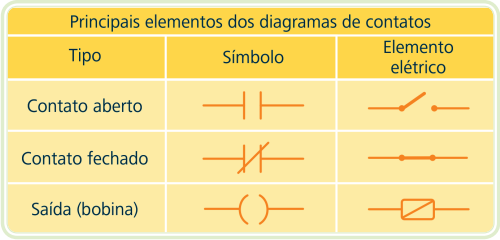
\includegraphics[width=\textwidth]{imagens/elemdiagcont.png}
    \caption{ELEMENTOS DO DIAGRAMA DE CONTATOS}
    \label{fig:elementos}
\end{figure}

As funções lógicas booleanas podem ser replicadas aplicando uma sequência de entradas pelo diagrama de contatos. Uma porta NOT é replicada posicionando um contato fechado e uma bobina. Uma porta OR É feita posicionando dois diagramas de contato aberto paralelos, ligados a uma bobina. A porta AND pode ser replicada posicionando dois diagramas de contato abertos em série, seguidos por uma bobina. Na figura ~\ref{fig:equivalencia}, as representações podem ser observadas.


\begin{figure}[h!]
    \centering
    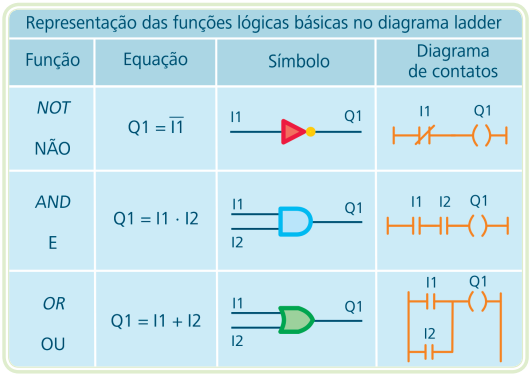
\includegraphics[width=\textwidth]{imagens/equivalportlogic.png}
    \caption{EQUIVALÊNCIA DAS PORTAS LÓGICAS EM LADDER}
    \label{fig:equivalencia}
\end{figure}

Outras funções existem para o diagrama de contatos. A função set é utilizada para manter uma bobina acessa após ter sido acionada, mesmo que o sinal não seja mais captado. Funciona como uma alavanca, enquanto normalmente funciona como um botão pressionado. A função reset serve para desacionar uma bobina que estava acessa pela função set. É como desligar a alavanca acionada previamente. Essas funções podem ser vistas na figura 3, em sua representação ladder.  

Um temporizador pode ser utilizado para acionar ou desligar uma saída de acordo com um tempo previamente programado. Pode então ser usada para acionar algo após um tempo do acionamento, ou desligá-lo após um tempo. Um contador serve para ativar uma saída após um certo número de ocorrências de algo, de acordo com sua programação. Pode ser usado então para ativar algo após um sinal ter sido captado um certo número de vezes. Estas funções também podem ser vistas na figura ~\ref{fig:funcoes}, em sua representação ladder.

\begin{figure}[h]
    \centering
    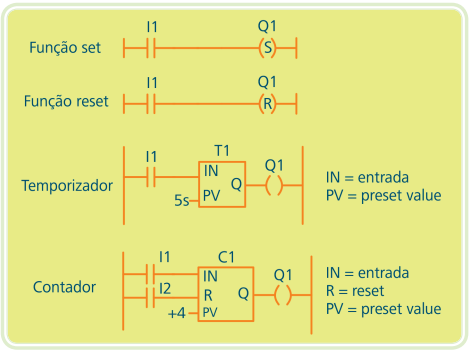
\includegraphics[width=\textwidth]{imagens/funcextras.png}
    \caption{OUTRAS FUNÇÕES EM LADDER}
    \label{fig:funcoes}
\end{figure}


\section{Exemplo prático: Plataforma de Petróleo}
No contexto de Ciência da Computação, automação é uma área com enorme impacto prático: podemos automatizar monitoramento, controle, processamento de dados, integração de sensores, geração de alertas, e outros. Para o estudo de um exemplo prático, podemos considerar a plataforma de Petróleo P-70 que trabalha no pré-sal, de Atapu, na Bacia de Santos, possuindo 316 metros de comprimento. Ela é uma plataforma de FPSO (Floating Production Storage and Offloading), ou Unidade Flutuante de Produção, Armazenamento e transferência de Óleo e Gás. Esse tipo de plataforma flutua no mar, cerca de 2 km acima do leito marinho, como um navio, sendo presa ao fundo do mar com algumas âncoras.   

Em uma plataforma, existem vários poços, estes que são responsáveis pela coleta do petróleo, ou para a injeção de água e gás (Para repor o óleo removido). Quando o óleo é retirado, é transportado por dutos, chamados de Flow em sua parte inferior (Fundo do mar) e de Risers em sua parte superior (Perto da plataforma). Na plataforma de exemplo, cada poço é ligado por 3 vias: Uma de produção, por onde é coletado o óleo; Uma de serviço que faz várias coisas, dentre elas a injeção de gás; E uma umbilical, pela qual é realizada a leitura e controle dos diversos sensores, além da injeção de produtos químicos no óleo, para evitar que os tubos sejam entupidos devido a uma reação da água salgada retirada. 

O petróleo passa por vários processos após ser retirado. O primeiro é a separação de gás e água em um vaso de separação. O gás separado pode ser vendido, para reinjeção nos poços ou até mesmo para a alimentação da energia da plataforma. Primeiro, o gás retirado deve ir para a compressão, aumentando a pressão do gás, para ir em seguida para a etapa de desidratação, removendo as moléculas de água através de uma peneira molecular, que as impede e deixa passar as moléculas de ar. Então, o gás carbônico é removido, pois não oferece valor, que então pode ser reinjetado no poço. A água removida pelo vaso de separação pode ser tratada para ser devolvida para o mar. 

O óleo ainda deve ir para uma outra separação, para a remoção da água, através de separação eletrostática, que puxa a água até ser possível a separar por gravidade. 

Petróleo é muito inflamável, então é necessário ter muito cuidado e controle sobre ele. Para isso, várias técnicas são adotadas. A mais importante é não deixar o oxigênio entrar nos tanques, que é uma operação complicada. Com a variação de temperatura durante o dia resulta na variação da pressão dentro dos tanques, sendo preciso aliviar o gás que está dentro caso esteja muito alta, e quando está mais baixa, é corrido o risco de entrar ar junto com oxigênio. Para isso, um gás inerte (Que não tem reações com o combustível) é injetado, não deixando que ocorra um incêndio.  

Cada plataforma tem uma chaminé chamada de Flare, onde são queimados os gases que sobraram dos processos, mas que deve ser feito ao mínimo possível. Também possuem a funcionalidade de servirem como um equipamento de segurança, para caso uma quantidade de gás precise ser dispensada de maneira ágil, quais são jogados para o Flare. 

A sala de controle da plataforma é onde se pode ser visualizado e realizada a leitura de todos os sensores, além de que permite controlá-los a distância. Por exemplo, é possível saber a temperatura de um poço, tanto quando ele está saindo do reservatório até quando ele chega na plataforma. A planta funciona de um modo automático, e os operadores interveem nos poços como um piloto de avião intervê em sua decolagem, com o resto sendo feito de modo automatizado. Para casos de emergência, existem vários botões para realizar a parada de diversos processos, de gerações e a parada total da plataforma. 

As áreas automatizadas em uma plataforma de petróleo são muitas, como: Para monitoramento ambiental e operacional, que pode utilizar de sensores para temperatura, pressão, nível de fluidos, composição de gás, vazamentos, integridade estrutural e outros. Estes sensores podem alimentar dashboards em tempo real. Permite detecção precoce de anomalias, menor risco de acidentes, melhor resposta a emergências. Para processo de separação e tratamento, podem ser utilizados 
controladores automáticos para válvulas, bombas, sistemas de injeção de químicos e ajuste automático de fluxo conforme sensores de qualidade. Traz otimização de eficiência, redução de desperdício, saída mais uniforme e estável.  

No tratamento de água potável e efluentes, podem existir a automatização do processo de dessalinização, remineralização, uso de UV, controle de vazão e monitoramento da qualidade (pH, turbidez etc.). Isso dá garantia de qualidade da água, economia de insumos, menor risco sanitário. Para a geração de energia e contingência	 podem existir sistemas automáticos de troca entre fonte principal e geradores de emergência, monitoramento de falhas elétricas e controle de carga. Garante resiliência energética, operação contínua sem falhas críticas. 

Na área de segurança, coisas como a detecção automática de gases inflamáveis, controle de inertização dos tanques, alarmes, sistemas de flare automáticos e evacuação assistida podem ser automatizadas, trazendo maior segurança dos trabalhadores, resposta rápida em situações de risco.  Na gestão de resíduos sólidos e líquidos, podem existir roteiros automáticos para tratamento, armazenagem e disposição; Monitoramento da conformidade com padrões ambientais, trazendo menos impacto ambiental e cumprimento das normas regulatórias.  

No entanto, muitas dificuldades também podem ser encontradas, que necessitam de atenção, como: Condições ambientais adversas: corrosão, umidade, salinidade podem afetar sensores e dispositivos eletrônicos; Acesso difícil para manutenção: se algo quebra, levar peças ou técnicos pode demorar. Isso impõe forte necessidade de robustez e redundância;  

Também podem ser problemas: Segurança crítica: automação mal implementada pode trazer riscos sérios (ex. controle incorreto de válvulas de gás ou falha nos sistemas de flare); Integração de sistemas legados: muitos equipamentos podem ser antigos ou usar protocolos diferentes, o que exige interfaces ou adaptação; Latência e confiabilidade de comunicações: em ambientes marítimos, garantir comunicação (dados) contínua pode ser desafio. 

A energização da plataforma de exemplo é realizada por 4 termelétricas de 25 MW (Megawatt) cada. Sua alimentação é realizada com gás natural ou com óleo diesel. As turbinas dos geradores são aeroderivadas (semelhante a uma turbina de um motor de avião a jato). O ar quente que sai delas é aproveitado para esquentar a água utilizada pela planta. Existe um gerador de emergência para caso ocorra falha nos outros. É um motor a diesel com 16 cilindros e consegue gerar 1.8 MW. 

A água potável utilizada é tratada na própria plataforma. É coletada a água do mar e o sal é removido através de vácuo, então é realizada a remineralização, para então passar por um tratamento ultravioleta, e após são armazenadas em um tanque pressurizado com ar comprimido. A água já utilizada não é imediatamente despejada. Primeiro, ela é tratada na própria plataforma. A parte líquida é então devolvida para o mar, e a parte sólida é guardada para ser devolvida para o continente.  

O nível mais baixo da plataforma	 está aproximadamente 10 metros abaixo do nível do mar, e é onde ficam as bombas para realizar a coleta da água salgada para prover para a plataforma.

\section{Conclusão}

A automação industrial é uma ampla, com muitos elementos e dispositivos. Desta forma, com este estudo, algum desses elementos foram apresentados. A automação pode estar presente e ser implementada de várias maneiras, podendo ser lidado com grandezas e valores discretos e contínuos. A captação desses valores pode ser feita através de uma variedade de sensores, cada um específico para alguma situação, quais captam informações sobre o ambiente em que estão inseridos, e reagem de alguma maneira, produzindo uma saída. Os relés e contatores podem ser utilizados para comandar e controlar circuitos elétricos e eletromecânicos, respectivamente. Os circuitos controlados podem ser vários, incluindo os motores CC e de passo, assim como as eletroválvulas hidráulicas e pneumáticas. Com a evolução da automação, foram desenvolvidos os CLP, que são dispositivos capazes de serem programáveis, o que os tornou muito importantes e altamente utilizados na automação. Capazes de captar sinais de entrada, e através da programação gerar resultados derivados de lógicas, cálculos aritméticos, de temporização e outras, atuam no sistema por meio de suas saídas, podendo ativar uma variedade de dispositivos como motores e válvulas.


\section{Referências}

ROGGIA, Leandro, FUENTES, Rodrigo Cardozo. Automação Industrial. rede e-Tec Brasil. Santa Maria, RS: Colégio Técnico Industrial de Santa Maria, 2016. 

\end{document}
